\subsection{Combining type models}
\label{subsec:transformation_framework:type_models_and_type_graphs:combining_type_models}

The structure of \cref{fig:transformation_framework:type_models_and_type_graphs:structure_type_models_graphs} shows that the type models $Tm_A$ and $Tm_B$ are combined into one type model $Tm_{AB}$. This section provides the definition of this combination and its corresponding theorems. Please note that the definitions presented here are as generic as possible, and do not actively take into account that $Tm_{A}$ and $Tm_{B}$ are mostly distinct. This bit of information is added later as part of a theorem and proof.

\begin{defin}[Combination function on type models]
\label{defin:transformation_framework:type_models_and_type_graphs:combining_type_models:combine}
$\mathrm{combine}$ is a binary function on two type models which combines two type models into one type model. It is defined as follows:
\begin{align*}
\mathrm{combine}(Tm_A, Tm_B) = \langle&
Class = Class_{Tm_A} \cup Class_{Tm_B} \\&
Enum = Enum_{Tm_A} \cup Enum_{Tm_B} \\&
UserDataType = UserDataType_{Tm_A} \cup UserDataType_{Tm_B} \\&
Field = Field_{Tm_A} \cup Field_{Tm_B} \\&
\mathrm{FieldSig} = \mathrm{fieldsig\_\!combine}(Tm_A, Tm_B) \\&
EnumValue = EnumValue_{Tm_A} \cup EnumValue_{Tm_B} \\&
Inh = Inh_{Tm_A} \cup Inh_{Tm_B} \\&
Prop = \mathrm{prop\_\!combine}(Tm_A, Tm_B) \\&
Constant = Constant_{Tm_A} \cup Constant_{Tm_B} \\&
\mathrm{ConstType} = \mathrm{consttype\_\!combine}(Tm_A, Tm_B)\rangle
\end{align*}

In which $\mathrm{fieldsig\_\!combine}$ is given as part of \cref{defin:transformation_framework:type_models_and_type_graphs:combining_type_models:fieldsig_combine}, $\mathrm{prop\_\!combine}$ as part of \cref{defin:transformation_framework:type_models_and_type_graphs:combining_type_models:prop_combine} and $\mathrm{consttype\_\!combine}$ as part of \cref{defin:transformation_framework:type_models_and_type_graphs:combining_type_models:consttype_combine}.
\isabellelref{tmod_combine}{Ecore.Type_Model_Combination}
\end{defin}

The combination of two type models is rather simple in its definition, at least for all the sets defined as part of a type model. Intuitively, the definition makes sense. To combine two type models, we need the types from both type models, so we merge the classes, enumerations types, enumeration values and user-defined data types. The constants should also be preserved, so these are merged too. To preserve all attributes and relations, we merge the set of fields and the inheritance relation as well.

Merging the different functions is done by using a new function. First, the combination of field signatures will be discussed.

\begin{defin}[Combination function for field signatures]
\label{defin:transformation_framework:type_models_and_type_graphs:combining_type_models:fieldsig_combine}
$\mathrm{fieldsig\_\!combine}$ is a partial function on two type models which returns a new function $Field_{Tm_{AB}} \Rightarrow (Type_{Tm_{AB}} \times \mathbb{M})$. It is defined as follows:
\begin{multline*}
    \mathrm{fieldsig\_\!combine}(Tm_{A}, Tm_{B}, f) = \\
        \begin{cases}
        s & \mathrm{if } f \in Field_{Tm_A} \cap Field_{Tm_B} \land \mathrm{type}_{Tm_A}(f) = \mathrm{type}_{Tm_B}(f) \\
        \mathrm{FieldSig}_{Tm_A}(f) & \mathrm{if } f \in Field_{Tm_A} \setminus Field_{Tm_B} \\
        \mathrm{FieldSig}_{Tm_B}(f) & \mathrm{if } f \in Field_{Tm_B} \setminus Field_{Tm_A}
    \end{cases}
\end{multline*}
where
\begin{equation*}
\begin{split}
    s = \bigg(\mathrm{type}_{Tm_A}(f), \Big(\max\left(\mathrm{lower}(\mathrm{FieldSig}_{Tm_A}(f)), \mathrm{lower}(\mathrm{FieldSig}_{Tm_B}(f))\right) ..\\ \min\left(\mathrm{upper}(\mathrm{FieldSig}_{Tm_A}(f)), \mathrm{upper}(\mathrm{FieldSig}_{Tm_B}(f))\right)\Big)\bigg)
\end{split}
\end{equation*}
\isabellelref{tmod_combine_fieldsig}{Ecore.Type_Model_Combination}
\end{defin}

Although the above definition looks quite complex, the intuition behind it is straightforward. For a field that only occurs in type model $Tm_A$, the field signature over from $Tm_A$ is copied. For a field that only occurs in $Tm_B$, the field signature from $Tm_B$ is copied. In the case that a field occurs in both $Tm_A$ and $Tm_B$, it should be the case that the type of the fields is the same. If this is indeed the case, the field type is copied, and a new multiplicity is created. This multiplicity takes the maximum of the lower bounds of the field in $Tm_A$ and $Tm_B$ as new lower bound, and the minimum of the upper bounds of the field in $Tm_A$ and $Tm_B$ as new upper bound.

\begin{figure}
    \centering
    \begin{subfigure}{0.45\textwidth}
        \centering
        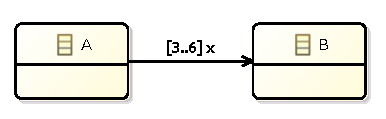
\includegraphics{images/04_transformation_framework/type_models_combination/fieldsig_combine_tmod1.pdf}
        \caption{First type model $Tm_A$}
        \label{fig:transformation_framework:type_models_and_type_graphs:combining_type_models:fieldsig_combine_tmod1}
    \end{subfigure}
    \begin{subfigure}{0.45\textwidth}
        \centering
        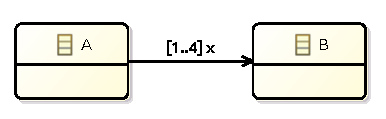
\includegraphics{images/04_transformation_framework/type_models_combination/fieldsig_combine_tmod2.pdf}
        \caption{Second type model $Tm_A$}
        \label{fig:transformation_framework:type_models_and_type_graphs:combining_type_models:fieldsig_combine_tmod2}
    \end{subfigure}
    \par\medskip
    \begin{subfigure}{\textwidth}
        \centering
        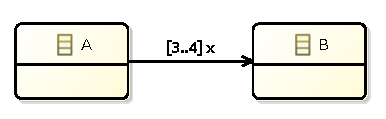
\includegraphics{images/04_transformation_framework/type_models_combination/fieldsig_combine_tmod12.pdf}
        \caption{Combined type model $Tm_{AB}$}
        \label{fig:transformation_framework:type_models_and_type_graphs:combining_type_models:fieldsig_combine_tmod12}
    \end{subfigure}
    \caption{Combination of field signatures when field is present in both type models}
    \label{fig:transformation_framework:type_models_and_type_graphs:combining_type_models:fieldsig_combine}
\end{figure}

An example of the combination of two field signatures in the case of a field being present in both $Tm_A$ and $Tm_B$ is given in \cref{fig:transformation_framework:type_models_and_type_graphs:combining_type_models:fieldsig_combine}. It is possible to combine the field $\type{x}$, since in both $Tm_A$ and $Tm_B$ field $\type{x}$ references class type $\type{B}$. The multiplicity for both field signatures is different and is combined as defined. The maximum of the lower bounds is taken, which results in $\max(3, 1) = 3$. Furthermore, the minimum of the upper bounds is taken, which results in $\min(6, 4) = 4$. Therefore the multiplicity of $\type{x}$ in $Tm_{AB}$ will become $3..4$.

Besides a function for field signatures, a type model also defines a function for constant types. The combination of constant types is discussed in the next definition.

\begin{defin}[Combination function for constant types]
\label{defin:transformation_framework:type_models_and_type_graphs:combining_type_models:consttype_combine}
$\mathrm{consttype\_\!combine}$ is a partial function on two type models which returns a new function \\$Constant_{Tm_{AB}} \Rightarrow Type_{Tm_{AB}}$. It is defined as follows:
\begin{multline*}
    \mathrm{consttype\_\!combine}(Tm_{A}, Tm_{B}, c) = \\
        \begin{cases}
        \mathrm{ConstType}_{Tm_A}(c) & \mathrm{if}\ c \in Constant_{Tm_A} \cap Constant_{Tm_B} \land \mathrm{ConstType}_{Tm_A}(c) = \mathrm{ConstType}_{Tm_B}(c) \\
        \mathrm{ConstType}_{Tm_A}(c) & \mathrm{if}\ c \in Constant_{Tm_A} \setminus Constant_{Tm_B} \\
        \mathrm{ConstType}_{Tm_B}(c) & \mathrm{if}\ c \in Constant_{Tm_B} \setminus Constant_{Tm_A}
    \end{cases}
\end{multline*}
\isabellelref{tmod_combine_const_type}{Ecore.Type_Model_Combination}
\end{defin}

The definition of the combination of constant types is similar to the combination of field signatures. The combination of constant types is less complicated because there is no notion of multiplicities involved. By definition, if a constant only occurs in $Tm_{A}$, the constant type of $Tm_{A}$ is copied. For constants that only occur in $Tm_{B}$, the constant type of $Tm_{B}$ is copied. In case that a constant occurs in both $Tm_{A}$ and $Tm_{B}$, the constant is copied if the constant types for that constant are the same in both $Tm_{A}$ and $Tm_{B}$.

The last definition that remains to be given is the definition of combining the set of properties. The set of properties cannot be united by merely taking the union of $Prop_{Tm_A}$ and $Prop_{Tm_B}$ since this might invalidate the satisfaction of these properties on the level of an instance graph. Instead, the inductive set $\mathrm{prop\_\!combine}$ is defined to specify under which circumstances a property can be combined.

\begin{defin}[Combination of model properties]
\label{defin:transformation_framework:type_models_and_type_graphs:combining_type_models:prop_combine}
$\mathrm{prop\_\!combine}(Tm_A, Tm_B)$ is defined as a subset of $Prop_{Tm_A} \cup Prop_{Tm_B}$. The contents of the set are then defined as follows:

For $\type{abstract}$ properties:
\begin{mathpar}
    \inferrule{[ \type{abstract}, c ] \in Prop_{Tm_A} \\ c \not\in Class_{Tm_B}}{[ \type{abstract}, c ] \in \mathrm{prop\_\!combine}(Tm_A, Tm_B)}
    \and
    \inferrule{[ \type{abstract}, c ] \in Prop_{Tm_B} \\ c \not\in Class_{Tm_A}}{[ \type{abstract}, c ] \in \mathrm{prop\_\!combine}(Tm_A, Tm_B)}
    \and
    \inferrule{[ \type{abstract}, c ] \in Prop_{Tm_A} \\ [ \type{abstract}, c ] \in Prop_{Tm_B}}{[ \type{abstract}, c ] \in \mathrm{prop\_\!combine}(Tm_A, Tm_B)}
\end{mathpar}

For $\type{containment}$ properties:
\begin{mathpar}
    \inferrule{[ \type{containment}, r ]\in Prop_{Tm_A}}{[ \type{containment}, r ]\in \mathrm{prop\_\!combine}(Tm_A, Tm_B)}
    \and
    \inferrule{[ \type{containment}, r ]\in Prop_{Tm_B}}{[ \type{containment}, r ]\in \mathrm{prop\_\!combine}(Tm_A, Tm_B)}
\end{mathpar}

For $\type{defaultValue}$ properties:
\begin{mathpar}
    \inferrule{[ \type{defaultValue}, f, v ]\in Prop_{Tm_A} \\ f \not\in Field_{Tm_B}}{[ \type{defaultValue}, f, v ]\in \mathrm{prop\_\!combine}(Tm_A, Tm_B)}
    \and
    \inferrule{[ \type{defaultValue}, f, v ]\in Prop_{Tm_B} \\ f \not\in Field_{Tm_A}}{[ \type{defaultValue}, f, v ]\in \mathrm{prop\_\!combine}(Tm_A, Tm_B)}
    \and
    \inferrule{[ \type{defaultValue}, f, v ]\in Prop_{Tm_A} \\ [ \type{defaultValue}, f, v ]\in Prop_{Tm_B}}{[ \type{defaultValue}, f, v ]\in \mathrm{prop\_\!combine}(Tm_A, Tm_B)}
\end{mathpar}

For $\type{identity}$ properties:
\begin{mathpar}
    \inferrule{[ \type{identity}, c, A ]\in Prop_{Tm_A} \\ c \not\in Class_{Tm_B}}{[ \type{identity}, c, A ]\in \mathrm{prop\_\!combine}(Tm_A, Tm_B)}
    \and
    \inferrule{[ \type{identity}, c, A ]\in Prop_{Tm_B} \\ c \not\in Class_{Tm_A}}{[ \type{identity}, c, A ]\in \mathrm{prop\_\!combine}(Tm_A, Tm_B)}
    \and
    \inferrule{[ \type{identity}, c, A ]\in Prop_{Tm_A} \\ [ \type{identity}, c, A ]\in Prop_{Tm_B}}{[ \type{identity}, c, A ]\in \mathrm{prop\_\!combine}(Tm_A, Tm_B)}
\end{mathpar}

For $\type{keyset}$ properties:
\begin{mathpar}
    \inferrule{[ \type{keyset}, r, A ]\in Prop_{Tm_A} \\ r \not\in Field_{Tm_B}}{[ \type{keyset}, r, A ]\in \mathrm{prop\_\!combine}(Tm_A, Tm_B)}
    \and
    \inferrule{[ \type{keyset}, r, A ]\in Prop_{Tm_B} \\ r \not\in Field_{Tm_A}}{[ \type{keyset}, r, A ]\in \mathrm{prop\_\!combine}(Tm_A, Tm_B)}
    \and
    \inferrule{[ \type{keyset}, r, A ]\in Prop_{Tm_A} \\ [ \type{keyset}, r, A ]\in Prop_{Tm_B}}{[ \type{keyset}, r, A ]\in \mathrm{prop\_\!combine}(Tm_A, Tm_B)}
\end{mathpar}

For $\type{opposite}$ properties:
\begin{mathpar}
    \inferrule{[ \type{opposite}, r1, r2 ]\in Prop_{Tm_A} \\ r1 \not\in Field_{Tm_B} \\ r2 \not\in Field_{Tm_B}}{[ \type{opposite}, r1, r2 ]\in \mathrm{prop\_\!combine}(Tm_A, Tm_B)}
    \and
    \inferrule{[ \type{opposite}, r1, r2 ]\in Prop_{Tm_B} \\ r1 \not\in Field_{Tm_A} \\ r2 \not\in Field_{Tm_A}}{[ \type{opposite}, r1, r2 ]\in \mathrm{prop\_\!combine}(Tm_A, Tm_B)}
    \and
    \inferrule{[ \type{opposite}, r1, r2 ]\in Prop_{Tm_A} \\ [ \type{opposite}, r1, r2 ]\in Prop_{Tm_B}}{[ \type{opposite}, r1, r2 ]\in \mathrm{prop\_\!combine}(Tm_A, Tm_B)}
\end{mathpar}

For $\type{readonly}$ properties:
\begin{mathpar}
    \inferrule{[ \type{readonly}, f ] \in Prop_{Tm_A} \\ f \not\in Field_{Tm_B}}{[ \type{readonly}, f ] \in \mathrm{prop\_\!combine}(Tm_A, Tm_B)}
    \and
    \inferrule{[ \type{readonly}, f ] \in Prop_{Tm_B} \\ f \not\in Field_{Tm_A}}{[ \type{readonly}, f ] \in \mathrm{prop\_\!combine}(Tm_A, Tm_B)}
    \and
    \inferrule{[ \type{readonly}, f ] \in Prop_{Tm_A} \\ [ \type{readonly}, f ] \in Prop_{Tm_B}}{[ \type{readonly}, f ] \in \mathrm{prop\_\!combine}(Tm_A, Tm_B)}
\end{mathpar}
\isabellelref{tmod_combine_prop}{Ecore.Type_Model_Combination}
\end{defin}

As can be seen from the definition of $\mathrm{prop\_\!combine}(Tm_A, Tm_B)$, properties are only copied under specific circumstances. For $\type{abstract}$ properties, it holds that a class is only abstract in the combination of $Tm_A$ and $Tm_B$ if the class is abstract in both $Tm_A$ and $Tm_B$ or if the class is abstract in one of them, and the class does not occur in the other. Intuitively, this makes sense for correctness. If a class is abstract in both type models, there will not be instances of that class in any of the combined instance models type by those type models. The same holds if the class only occurs in one of the type models, as an instance model cannot contain an instance of a class that is not present in its type model.

For the containment property, it holds that the containment property is always copied over. There are no other conditions here. If there is a containment property in $Prop_{Tm_A} \cup Prop_{Tm_B}$ it will also be in the combination of $Tm_A$ and $Tm_B$.

A default value property is copied over from one of the type models if the other type model does not have the corresponding field defined. Furthermore, a default value may be in the combination of properties of $Tm_A$ and $Tm_B$ if the field occurs in both, and both have the same constant set as the default value for the field. Intuitively, this last requirement makes sense. If we set a default value for a field within a type model, it should not change after combining the type model with another type model, as instance models might depend on the default value set for that field.

Identity properties follow a similar pattern to default value properties. An identity is copied over from one of the type models if the corresponding class is not defined in the other type model. Furthermore, an identity can be preserved if it is set for the same class and attributes in both type models. Again, intuitively, this is the desired solution. If a type model has a class of which a set of attributes can uniquely define the instances, then this should also be the case after the combination with another type model. Merging two sets of attributes might have preserved the identity property as well, but this would be a questionable decision from a practical standpoint, as this means that the identity of instances changes, which makes no sense in real-world scenarios.

The argumentation for identity properties also holds for keyset properties. Therefore these follow a similar pattern, in which the keyset properties of a type model are only copied if the corresponding field does not occur in the other type model, or if the keyset property for a field occurs with the same attributes in both type models.

The opposite property is preserved if it occurs in a type model, but the other type model does not define both of the corresponding fields. Alternatively, the property is preserved if it occurs in both type models with the same fields. All different ways to combine an opposite property would result in an invalid type model according to \cref{defin:formalisations:ecore_formalisation:type_models:type_model_consistency}, which is undesired.

The read-only properties follow a similar pattern to the abstract properties. If a field is read-only in both type models, then it is read-only in the combination. Furthermore, if a field is read-only in one of the type models and the field is not defined in the other type model, then the read-only property can be copied too.

\begin{figure}
    \centering
    \begin{subfigure}{\textwidth}
        \centering
        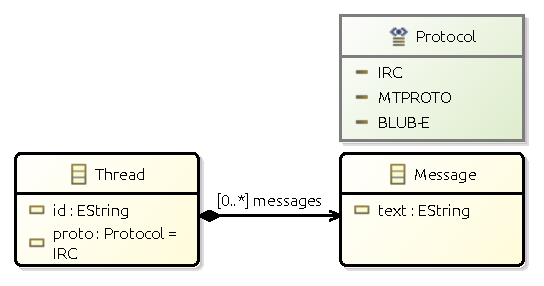
\includegraphics{images/04_transformation_framework/type_models_combination/chat_partial2.pdf}
        \caption{The chat application model $Tm_{Chat}$}
        \label{fig:transformation_framework:type_models_and_type_graphs:combining_type_models:combine_example_tmod1}
    \end{subfigure}
    \par\medskip
    \begin{subfigure}{\textwidth}
        \centering
        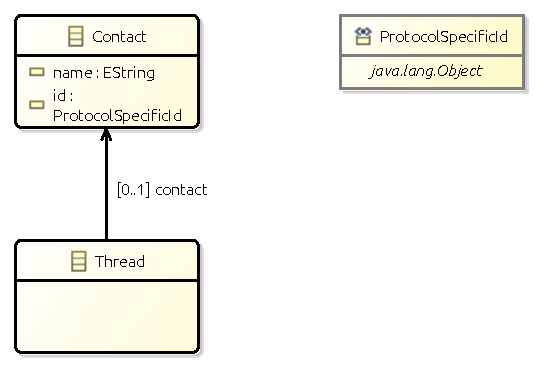
\includegraphics{images/04_transformation_framework/type_models_combination/chat_partial1.pdf}
        \caption{The contact extension model $Tm_{Extension}$}
        \label{fig:transformation_framework:type_models_and_type_graphs:combining_type_models:combine_example_tmod2}
    \end{subfigure}
    \par\medskip
    \begin{subfigure}{\textwidth}
        \centering
        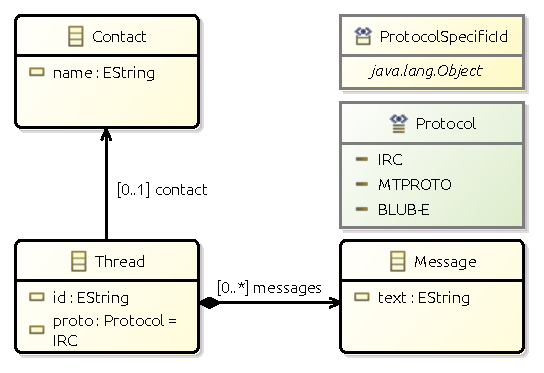
\includegraphics{images/04_transformation_framework/type_models_combination/chat_combined.pdf}
        \caption{The extended chat application model $Tm_{ChatExt}$}
        \label{fig:transformation_framework:type_models_and_type_graphs:combining_type_models:combine_example_tmod12}
    \end{subfigure}
    \caption{Example of the combination of type models}
    \label{fig:transformation_framework:type_models_and_type_graphs:combining_type_models:combine_example}
\end{figure}

With all definitions in place, it is possible to provide a larger example. Suppose the model of a multi-protocol chat application. It consists of $\type{Thread}$s of $\type{Message}$s. Since the application is multi-protocol, each $\type{Thread}$ can use one of the supported $\type{Protocol}$s. The formal definition of the model of such an application could be as follows:

\begin{align*}
Tm_{Chat} =\ &\langle&
Class =\ &\{ \type{.Message}, \type{.Thread} \} \\&&
Enum =\ &\{ \type{.Protocol} \} \\&&
UserDataType =\ &\{\} \\&&
Field =\ &\{
( \type{.Message}, \type{text} ), 
( \type{.Thread}, \type{id} ), 
( \type{.Thread}, \type{messages} ), 
( \type{.Thread}, \type{proto} )\} \\&&
\mathrm{FieldSig} =\ &\big\{
\big( ( \type{.Message}, \type{text} ), ( \type{string}, 1..1 ) \big), \big( ( \type{.Thread}, \type{id} ), ( \type{string}, 1..1 ) \big),\\&&& 
\big( ( \type{.Thread}, \type{messages} ), ( [ \type{seqof}, !\type{.Message} ], 0..\mstar ) \big),\\&&& 
\big( ( \type{.Thread}, \type{proto} ), ( \type{.Protocol}, 1..1 ) \big) \big)
\big\} \\&&
EnumValue =\ &\{
( \type{.Protocol}, \type{IRC} ), 
( \type{.Protocol}, \type{MTPROTO} ), 
( \type{.Protocol}, \type{BLUB\!-\!E} )\} \\&&
Inh =\ &\{\} \\&&
Prop =\ &\big\{
\big( \type{identity}, \type{.Message}, \{( \type{.Thread}, \type{id} )\} \big)
\big\} \\&&
Constant =\ &\{\} \\&&
\mathrm{ConstType} =\ &\{\}
\\&\rangle
\end{align*}

An visual representation of $Tm_{Chat}$ is included as  \cref{fig:transformation_framework:type_models_and_type_graphs:combining_type_models:combine_example_tmod1}. Now, assume a model that represents an extension to this application, adding support for $\type{Contact}$s. Each thread can belong to a $\type{Contact}$. A $\type{Contact}$ has a name and some identifier that is protocol specific. For that identifier, the user-defined data type $\type{ProtocolSpecificId}$ is introduced. This extension could formally be defined as:

\begin{align*}
Tm_{Extension} =\ &\langle&
Class =\ &\{ \type{.Contact}, \type{.Thread} \} \\&&
Enum =\ &\{\} \\&&
UserDataType =\ &\{ \type{.ProtocolSpecificId} \} \\&&
Field =\ &\{
( \type{.Contact}, \type{name} ), 
( \type{.Contact}, \type{id} ), 
( \type{.Thread}, \type{contact} )\} \\&&
\mathrm{FieldSig} =\ &\big\{
\big( ( \type{.Contact}, \type{name} ), ( \type{string}, 1..1 ) \big),\\&&& \big( ( \type{.Contact}, \type{id} ), ( \type{.ProtocolSpecificId}, 1..1 ) \big),\\&&& 
\big( ( \type{.Thread}, \type{contact} ), ( ?\type{.Contact}, 0..1 ) \big) \big)
\big\} \\&&
EnumValue =\ &\{\} \\&&
Inh =\ &\{\} \\&&
Prop =\ &\big\{
\big( \type{identity}, \type{.Contact}, \{( \type{.Contact}, \type{id} )\} \big)
\big\} \\&&
Constant =\ &\{\} \\&&
\mathrm{ConstType} =\ &\{\}
\\&\rangle
\end{align*}

The visual representation of the extension is included as \cref{fig:transformation_framework:type_models_and_type_graphs:combining_type_models:combine_example_tmod2}. Now, using \cref{defin:transformation_framework:type_models_and_type_graphs:combining_type_models:combine}, it is possible to combine these models into one model. This will yield the following model:

\begin{align*}
Tm_{ChatExt} =\ &\langle&
Class =\ &\{ \type{.Contact}, \type{.Message}, \type{.Thread} \} \\&&
Enum =\ &\{ \type{.Protocol} \} \\&&
UserDataType =\ &\{ \type{.ProtocolSpecificId} \} \\&&
Field =\ &\{
( \type{.Contact}, \type{name} ), 
( \type{.Contact}, \type{id} ),
( \type{.Message}, \type{text} ),\\&&&
( \type{.Thread}, \type{contact} ),
( \type{.Thread}, \type{id} ),
( \type{.Thread}, \type{messages} ),\\&&& 
( \type{.Thread}, \type{proto} )\} \\&&
\mathrm{FieldSig} =\ &\big\{
\big( ( \type{.Contact}, \type{name} ), ( \type{string}, 1..1 ) \big),\\&&& \big( ( \type{.Contact}, \type{id} ), ( \type{.ProtocolSpecificId}, 1..1 ) \big),\\&&& 
\big( ( \type{.Message}, \type{text} ), ( \type{string}, 1..1 ) \big),\\&&&
\big( ( \type{.Thread}, \type{contact} ), ( ?\type{.Contact}, 0..1 ) \big) \big),\\&&&
\big( ( \type{.Thread}, \type{id} ), ( \type{string}, 1..1 ) \big),\\&&& 
\big( ( \type{.Thread}, \type{messages} ), ( [ \type{seqof}, !\type{.Message} ], 0..\mstar ) \big),\\&&& 
\big( ( \type{.Thread}, \type{proto} ), ( \type{.Protocol}, 1..1 ) \big) \big)
\big\} \\&&
EnumValue =\ &\{
( \type{.Protocol}, \type{IRC} ), 
( \type{.Protocol}, \type{MTPROTO} ), 
( \type{.Protocol}, \type{BLUB\!-\!E} )\} \\&&
Inh =\ &\{\} \\&&
Prop =\ &\big\{
\big( \type{identity}, \type{.Contact}, \{( \type{.Contact}, \type{id} )\} \big),\\&&&
\big( \type{identity}, \type{.Message}, \{( \type{.Thread}, \type{id} )\} \big)
\big\} \\&&
Constant =\ &\{\} \\&&
\mathrm{ConstType} =\ &\{\}
\\&\rangle
\end{align*}

A visual representation of this combined model is included as \cref{fig:transformation_framework:type_models_and_type_graphs:combining_type_models:combine_example_tmod12}. The example perfectly shows why the combination of type models is useful: It allows for building larger models out of smaller building blocks. This is the exact goal of this definition within the transformation framework.

Although the definitions of the combination of type models are given, no mathematical properties or theorems are defined yet. Some mathematical properties hold for the combination of type models, that will be presented in the following theorems.

\begin{thm}[Commutativity of the combination of type models]
\label{defin:transformation_framework:type_models_and_type_graphs:combining_type_models:tmod_combine_commute}
Assume that $Tm_A$ and $Tm_B$ are type models, then the $\mathrm{combine}$ function is commutative:
\begin{equation*}
    \mathrm{combine}(Tm_A, Tm_B) = \mathrm{combine}(Tm_B, Tm_A)
\end{equation*}
\isabellelref{tmod_combine_commute}{Ecore.Type_Model_Combination}
\end{thm}

\begin{thm}[Associativity of the combination of type models]
\label{defin:transformation_framework:type_models_and_type_graphs:combining_type_models:tmod_combine_assoc}
Assume that $Tm_A$, $Tm_B$ and $Tm_C$ are type models, then the $\mathrm{combine}$ function is associative:
\begin{equation*}
    \mathrm{combine}(\mathrm{combine}(Tm_A, Tm_B), Tm_C) = \mathrm{combine}(Tm_A, \mathrm{combine}(Tm_B, Tm_C))
\end{equation*}
\isabellelref{tmod_combine_assoc}{Ecore.Type_Model_Combination}
\end{thm}

\begin{thm}[Idempotence of the combination of type models]
\label{defin:transformation_framework:type_models_and_type_graphs:combining_type_models:tmod_combine_idemp}
Assume that $Tm_A$ is a type model and that it is consistent in the sense of \cref{defin:formalisations:ecore_formalisation:type_models:type_model_consistency}. Then the following property holds:
\begin{equation*}
    \mathrm{combine}(Tm_A, Tm_A) = Tm_A
\end{equation*}
\isabellelref{tmod_combine_idemp_alt}{Ecore.Type_Model_Combination}
\end{thm}

These properties follow directly from \cref{defin:transformation_framework:type_models_and_type_graphs:combining_type_models:combine}, but the corresponding proofs will not be included here. It should be noted that these properties are indeed proven correct as part of this thesis, and the corresponding proofs are validated within Isabelle.

Besides these properties, the combination of type models also has an identity element. The empty type model represents this identity element, but it needs to be defined first:

\begin{defin}[Empty type model]
\label{defin:transformation_framework:type_models_and_type_graphs:combining_type_models:empty_type_model}
Let $Tm_{\epsilon}$ be the empty type model. $Tm_{\epsilon}$ is defined as:
\begin{align*}
Tm_{\epsilon} = \langle&
Class = \{\} \\&
Enum = \{\} \\&
UserDataType = \{\} \\&
Field = \{\} \\&
\mathrm{FieldSig} = undefined \\&
EnumValue = \{\} \\&
Inh = \{\} \\&
Prop = \{\} \\&
Constant = \{\} \\&
\mathrm{ConstType} = undefined\rangle
\end{align*}
\end{defin}

\begin{thm}[Correctness of the empty type model]
\label{defin:transformation_framework:type_models_and_type_graphs:combining_type_models:tmod_empty_correct}
The empty type model, $Tm_{\epsilon}$, is consistent with respect to
\cref{defin:formalisations:ecore_formalisation:type_models:type_model_consistency}.
\isabellelref{tmod_empty_correct}{Ecore.Type_Model}
\end{thm}

The proof for the correctness of the empty type model is trivial. Still, a validated version of this proof can be found within the Isabelle theories of this thesis.

As mentioned earlier, the empty type model acts as an identity element when combining two type models. The following theorem specifies this behaviour.

\begin{thm}[Identity of the combination of type models]
\label{defin:transformation_framework:type_models_and_type_graphs:combining_type_models:tmod_combine_identity}
Assume that $Tm_A$ is a type model and that it is consistent in the sense of \cref{defin:formalisations:ecore_formalisation:type_models:type_model_consistency}. Then $Tm_{\epsilon}$ acts as an identity element in the combination function:
\begin{equation*}
    \mathrm{combine}(Tm_{\epsilon}, Tm_A) = Tm_A
\end{equation*}
\isabellelref{tmod_combine_identity_alt}{Ecore.Type_Model_Combination}
\end{thm}

Once more, the proof of this theorem follows directly from the definition. Therefore, the corresponding proof will not be included here, but a validated version can be found within the Isabelle theories of this thesis.

A final desired property for the combination of type models is a correctness property. \cref{defin:transformation_framework:type_models_and_type_graphs:combining_type_models:tmod_combine_correct} defines the theorem under which the combination of type models is a consistent type model. Please note that this theorem is a generic theorem, which does not take into account that the type models are mostly distinct.

\begin{thm}[Consistency of the combination of type models]
\label{defin:transformation_framework:type_models_and_type_graphs:combining_type_models:tmod_combine_correct}
Assume that $Tm_A$ and $Tm_B$ are consistent type models in the sense of \cref{defin:formalisations:ecore_formalisation:type_models:type_model_consistency}. Furthermore, assume the following properties:
\begin{itemize}
    \item For all shared fields, the type is the same in both type models: $\forall f \in Field_{Tm_A} \cap Field_{Tm_B}\!: \mathrm{type}_{Tm_A}(f) = \mathrm{type}_{Tm_B}(f)$
    \item For all shared fields, the combination of the multiplicities is a valid multiplicity: $\forall f \in Field_{Tm_A} \cap Field_{Tm_B}\!: \max\big(\mathrm{lower}(\mathrm{FieldSig}_{Tm_A}(f)), \mathrm{lower}(\mathrm{FieldSig}_{Tm_B}(f))\big) .. \min\big(\mathrm{upper}(\mathrm{FieldSig}_{Tm_A}(f)),$\\ $\mathrm{upper}(\mathrm{FieldSig}_{Tm_B}(f))\big) \in \mathbb{M}$
    \item For all shared constants, the constant type is the same in both models: $\forall f \in Constant_{Tm_A} \cap Constant_{Tm_B}\!: \mathrm{ConstType}_{Tm_A}(f) = \mathrm{ConstType}_{Tm_B}(f)$
    \item Identifiers used for a class in $Tm_A$ cannot be used for an enumeration type or user-defined data type in $Tm_B$: $\forall c \in Class_{Tm_A}\!: c \not\in Enum_{Tm_B} \land c \not\in UserDataType_{Tm_B}$.
    \item Identifiers used for a class in $Tm_B$ cannot be used for an enumeration type or user-defined data type in $Tm_A$: $\forall c \in Class_{Tm_B}\!: c \not\in Enum_{Tm_A} \land c \not\in UserDataType_{Tm_A}$.
    \item Identifiers used for an enumeration type in $Tm_A$ cannot be used for a class or user-defined data type in $Tm_B$: $\forall c \in Enum_{Tm_A}\!: c \not\in Class_{Tm_B} \land c \not\in UserDataType_{Tm_B}$.
    \item Identifiers used for an enumeration type in $Tm_B$ cannot be used for a class or user-defined data type in $Tm_A$: $\forall c \in Enum_{Tm_B}\!: c \not\in Class_{Tm_A} \land c \not\in UserDataType_{Tm_A}$.
    \item Identifiers from $Tm_A$ may not be in the namespace of an identifier in $Tm_B$: $\forall x \in Class_{Tm_A} \cup Enum_{Tm_A} \cup UserDataType_{Tm_A}; y \in Class_{Tm_B} \cup Enum_{Tm_B} \cup UserDataType_{Tm_B}\!:$\\$x \text{ not in the namespace of } y$
    \item Identifiers from $Tm_B$ may not be in the namespace of an identifier in $Tm_A$: $\forall x \in Class_{Tm_B} \cup Enum_{Tm_B} \cup UserDataType_{Tm_B}; y \in Class_{Tm_A} \cup Enum_{Tm_A} \cup UserDataType_{Tm_A}\!:$\\$x \text{ not in the namespace of } y$
    \item The transitive closure of the inheritance relation is irreflexive: $(Inh_{Tm_A} \cup Inh_{Tm_B})^+$ is irreflexive
    \item For any superclass with an identity, the identity of the subclasses must be a superset of the identity of the superclass: $\forall c_1\ c_2\ A_1\ A_2\!: [ \type{identity}, c_1, A_1 ] \in \mathrm{prop\_\!combine}(Tm_A, Tm_B) \land [ \type{identity}, c_2, A_2 ] \in \mathrm{prop\_\!combine}(Tm_A, Tm_B) \land c_1 \neq c_2\ \land\ !c_1 \not\sqsubseteq_{Tm_A}\ !c_2\ \land\ !c_1 \not\sqsubseteq_{Tm_B}\ !c_2\ \land\ !c_1 \sqsubseteq_{\mathrm{combine}(Tm_A, Tm_B)}\ !c_2 \implies A \subseteq B$
    \item For all shared fields, if $Tm_{A}$ defines a default value, $Tm_{B}$ should define the same default value, and vice versa: $\forall f \in Field_{Tm_A} \cap Field_{Tm_B}\!: [ \type{defaultValue}, f, v ] \in Prop_{Tm_A} \Longleftrightarrow [ \type{defaultValue}, f, v ] \in Prop_{Tm_B}$.
    \item For all shared classes, if $Tm_{A}$ defines a identity, $Tm_{B}$ should define the same identity, and vice versa: $\forall c \in Class_{Tm_A} \cap Class_{Tm_B}\!: [ \type{identity}, c, A ] \in Prop_{Tm_A} \Longleftrightarrow [ \type{identity}, c, A ] \in Prop_{Tm_B}$.
    \item For all shared fields, if $Tm_{A}$ defines a keyset, $Tm_{B}$ should define the same keyset, and vice versa: $\forall r \in Field_{Tm_A} \cap Field_{Tm_B}\!: [ \type{keyset}, r, A ] \in Prop_{Tm_A} \Longleftrightarrow [ \type{keyset}, r, A ] \in Prop_{Tm_B}$.
    \item For all shared fields, if $Tm_{A}$ defines an opposite property, $Tm_{B}$ should define the same opposite property, and vice versa: $\forall r \in Field_{Tm_A} \cap Field_{Tm_B}\!: [ \type{opposite}, r, r' ] \in Prop_{Tm_A} \Longleftrightarrow [ \type{opposite}, r, r' ] \in Prop_{Tm_B}$
\end{itemize}

Then $\mathrm{combine}(Tm_A, Tm_B)$ is a consistent type model in the sense of \cref{defin:formalisations:ecore_formalisation:type_models:type_model_consistency}
\isabellelref{tmod_combine_correct}{Ecore.Type_Model_Combination}
\end{thm}

\begin{proof}
To proof that $\mathrm{combine}(Tm_A, Tm_B)$ is a consistent type model, it needs to be shown that\\ $\mathrm{combine}(Tm_A, Tm_B)$ gives rise to a valid structure for a type model and that \cref{defin:formalisations:ecore_formalisation:type_models:type_model_consistency} holds. For readability, define $Tm_{AB}$ to be $\mathrm{combine}(Tm_A, Tm_B)$.

\emph{Structural properties}
\begin{itemize}
    \item All elements of $Class_{Tm_{AB}}$ are elements of $Id$.
    
    Follows from $Class_{Tm_A} \subseteq Id$ and $Class_{Tm_B} \subseteq Id$.
    
    
    \item All elements of $Enum_{Tm_{AB}}$ are elements of $Id$.
    
    Follows from $Enum_{Tm_A} \subseteq Id$ and $Enum_{Tm_B} \subseteq Id$.
    
    
    \item All elements of $UserDataType_{Tm_{AB}}$ are elements of $Id$.
    
    Follows from $UserDataType_{Tm_A} \subseteq Id$ and $UserDataType_{Tm_B} \subseteq Id$.
    
    
    \item All elements of $Field_{Tm_{AB}}$ are elements of $(Class_{Tm_{AB}} \times Name)$.
    
    Follows from $Field_{Tm_A} \subseteq (Class_{Tm_A} \times Name)$ and $Field_{Tm_B} \subseteq (Class_{Tm_B} \times Name)$. To complete the proof, use $Class_{Tm_{AB}} = Class_{Tm_A} \cup Class_{Tm_B}$.
    
    
    \item For each field $f$, $\mathrm{FieldSig}_{Tm_{AB}}(f)$ must be an element of $(Type_{Tm_{AB}} \times \mathbb{M})$.
    
    First, note that $Type_{Tm_{AB}} = Type_{Tm_A} \cup Type_{Tm_B}$\\(see \isabelleref{tmod_combine_type}{Ecore.Type_Model_Combination}).
    
    If $f \in Field_{Tm_A} \setminus Field_{Tm_B}$, then $\mathrm{FieldSig}_{Tm_{AB}}(f) \in (Type_{Tm_{AB}} \times \mathbb{M})$.
    
    Similarly, if $f \in Field_{Tm_B} \setminus Field_{Tm_A}$, then $\mathrm{FieldSig}_{Tm_{AB}}(f) \in (Type_{Tm_{AB}} \times \mathbb{M})$. 
    
    If $f \in Field_{Tm_A} \cap Field_{Tm_B}$, then $\mathrm{type}_{Tm_A}(f) = \mathrm{type}_{Tm_B}(f)$ by assumption. Also, the combined multiplicity is correct by assumption. Therefore $\mathrm{FieldSig}_{Tm_{AB}}(f) \in (Type_{Tm_{AB}} \times \mathbb{M})$.
    
    
    \item All elements of $EnumValue_{Tm_{AB}}$ are elements of $(Enum_{Tm_{AB}} \times Name)$.
    
    Follows from $EnumValue_{Tm_A} \subseteq (Enum_{Tm_A} \times Name)$ and $EnumValue_{Tm_B} \subseteq (Enum_{Tm_B} \times Name)$. To complete the proof, use $Enum_{Tm_{AB}} = Enum_{Tm_A} \cup Enum_{Tm_B}$.
    
    
    \item All elements of $Inh_{Tm_{AB}}$ are elements of $(Class_{Tm_{AB}} \times Class_{Tm_{AB}})$.
    
    Follows from $Inh_{Tm_A} \subseteq (Class_{Tm_A} \times Class_{Tm_A})$ and $Inh_{Tm_B} \subseteq (Class_{Tm_B} \times Class_{Tm_B})$. Furthermore, $Class_{Tm_{AB}} = Class_{Tm_A} \cup Class_{Tm_B}$.
    
    
    \item All elements of $Prop_{Tm_{AB}}$ are elements of $Property_{Tm_{AB}}$.
    
    Make a case distinction for the different possible properties.
    \begin{itemize}
        \item For $[ \type{abstract}, c ] \in Prop_{Tm_{AB}}$, use the fact that $c \in Class_{Tm_A} \cup Class_{Tm_B}$. Therefore, $[ \type{abstract}, c ] \in Property_{Tm_{AB}}$.
        
        \item For $[ \type{containment}, r ] \in Prop_{Tm_{AB}}$, use the fact that $Rel_{Tm_{AB}} = Rel_{Tm_A} \cup Rel_{Tm_B}$ (see \isabelleref{tmod_combine_rel}{Ecore.Type_Model_Combination}). Then have $[ \type{containment}, r ] \in Property_{Tm_{AB}}$.
        
        \item For $[ \type{defaultValue}, f, v ] \in Prop_{Tm_{AB}}$, use the fact that $f \in Field_{Tm_A} \cup Field_{Tm_B}$ and $v \in Constant_{Tm_A} \cup Constant_{Tm_B}$. Using a case disinction on the combination of properties, it is possible to show that $\mathrm{ConstType}_{Tm_{AB}}(v) \sqsubseteq_{Tm_{AB}} \mathrm{type}_{Tm_{AB}}(f)$. Therefore, $[ \type{defaultValue}, f, v ] \in Property_{Tm_{AB}}$.
        
        \item For $[ \type{identity}, c, A ] \in Prop_{Tm_{AB}}$, use the fact that $c \in Class_{Tm_A} \cup Class_{Tm_B}$ and $A \subseteq fields_{Tm_A} \lor A \subseteq fields_{Tm_B}$. Then have that $A \subseteq fields_{Tm_{AB}}$ Therefore, $[ \type{identity}, c, A ] \in Property_{Tm_{AB}}$.
        
        \item For $[ \type{keyset}, r, A ] \in Prop_{Tm_{AB}}$, use the fact that $Rel_{Tm_{AB}} = Rel_{Tm_A} \cup Rel_{Tm_B}$ (see \isabelleref{tmod_combine_rel}{Ecore.Type_Model_Combination}) to show $r \in Rel_{Tm_{AB}}$. Also use the fact that $Attr_{Tm_{AB}} = Attr_{Tm_A} \cup Attr_{Tm_B}$ to show $A \subseteq Attr_{Tm_{AB}}$ (see \isabelleref{tmod_combine_attr}{Ecore.Type_Model_Combination}). Because types are preserved after combining, it is possible to show that $\forall f \in A\!: \mathrm{uncontainer}(\mathrm{type}_{Tm_{AB}}(r)) \sqsubseteq_{Tm_{AB}} \mathrm{class}_{Tm_{AB}}(f)$. Furthermore, $\mathrm{type}_{Tm_{AB}}(r) \in (\{ \type{setof}, \type{ordof} \} \times ClassType_{Tm_{AB}})$. Therefore, $[ \type{keyset}, r, A ] \in Property_{Tm_{AB}}$.
        
        \item For $[ \type{opposite}, r, r' ] \in Prop_{Tm_{AB}}$, use the fact that $Rel_{Tm_{AB}} = Rel_{Tm_A} \cup Rel_{Tm_B}$ (see \isabelleref{tmod_combine_rel}{Ecore.Type_Model_Combination}) to show $r \in Rel_{Tm_{AB}}$ and $r' \in Rel_{Tm_{AB}}$. Because types are preserved after combining, it is possible to show that $!c1 \sqsubseteq_{Tm_{AB}} \mathrm{uncontainer}(\mathrm{type}_{Tm_{AB}}(r'))$, $!c2 \sqsubseteq_{Tm_{AB}} \mathrm{uncontainer}(\mathrm{type}_{Tm_{AB}}(r))$,\\ $\mathrm{type}_{Tm_{AB}}(r) \not\in \{ \type{bagof}, \type{seqof} \} \times Type_{Tm_{AB}}$ and finally $type_{Tm_{AB}}(r') \not\in \{ \type{bagof}, \type{seqof} \} \times Type_{Tm_{AB}}$. Therefore, $[ \type{opposite}, r, r' ] \in Property_{Tm_{AB}}$.
        
        \item For $[ \type{readonly}, f ] \in Prop_{Tm_{AB}}$, use the fact that $f \in Field_{Tm_A} \cup Field_{Tm_B}$. Therefore, $[ \type{readonly}, f ] \in Property_{Tm_{AB}}$.
    \end{itemize}
    
    
    \item All elements of $Constant_{Tm_{AB}}$ are elements of $Id$.
    
    Follows from $Constant_{Tm_A} \subseteq Id$ and $Constant_{Tm_B} \subseteq Id$.
    
    
    \item For each constant $c$, $\mathrm{ConstType}_{Tm_{AB}}(c)$ must be an element of $Type_{Tm_{AB}}$.
    
    First, note that $Type_{Tm_{AB}} = Type_{Tm_A} \cup Type_{Tm_B}$\\(see \isabelleref{tmod_combine_type}{Ecore.Type_Model_Combination}).
    
    If $c \in Constant_{Tm_A} \setminus Constant_{Tm_B}$, then $\mathrm{ConstType}_{Tm_{AB}}(f) \in Type_{Tm_{AB}}$.
    
    Similarly, if $c \in Constant_{Tm_B} \setminus Constant_{Tm_A}$, then $\mathrm{ConstType}_{Tm_{AB}}(c) \in Type_{Tm_{AB}}$.
    
    If $c \in Constant_{Tm_A} \cap Constant_{Tm_B}$, then $\mathrm{ConstType}_{Tm_A}(c) = \mathrm{ConstType}_{Tm_B}(c)$ by assumption. Therefore $\mathrm{ConstType}_{Tm_{AB}}(c) \in Type_{Tm_{AB}}$.
    
    
    \item $Class_{Tm_{AB}}$, $DataType$, $Enum_{Tm_{AB}}$ and $UserDataType_{Tm_{AB}}$ are pairwise disjoint.
    
    Notice that $Class_{Tm_{A}}$, $DataType$, $Enum_{Tm_{A}}$, $UserDataType_{Tm_{A}}$ are pairwise disjoint. Also, $Class_{Tm_{B}}$, $DataType$, $Enum_{Tm_{B}}$, $UserDataType_{Tm_{B}}$ are pairwise disjoint.
    
    Use that $Class_{Tm_{AB}} = Class_{Tm_{A}} \cup Class_{Tm_{B}}$, $Enum_{Tm_{AB}} = Enum_{Tm_{A}} \cup Enum_{Tm_{B}}$ and\\ $UserDataType_{Tm_{AB}} = UserDataType_{Tm_{A}} \cup UserDataType_{Tm_{B}}$. Use this to split the possible cases.
    
    Only the case where one element is from $Class_{Tm_{A}} \cup Enum_{Tm_{A}} \cup UserDataType_{Tm_{A}}$ and one element is from $Class_{Tm_{B}} \cup Enum_{Tm_{B}} \cup UserDataType_{Tm_{B}}$ cannot be proven directly. For this case, the proof follows from the assumptions.
    
    
    \item None of the elements in $Class_{Tm_{AB}}$, $DataType$, $Enum_{Tm_{AB}}$ and $UserDataType_{Tm_{AB}}$ may be in the namespace of another element in that set.
    
    Use that $Class_{Tm_{AB}} = Class_{Tm_{A}} \cup Class_{Tm_{B}}$, $Enum_{Tm_{AB}} = Enum_{Tm_{A}} \cup Enum_{Tm_{B}}$ and\\ $UserDataType_{Tm_{AB}} = UserDataType_{Tm_{A}} \cup UserDataType_{Tm_{B}}$. Use this to split the possible cases.
    
    It is not possible to directly proof the cases where the identifier comes from $Class_{Tm_{A}} \cup Enum_{Tm_{A}} \cup UserDataType_{Tm_{A}}$ and the namespace comes from $Class_{Tm_{B}} \cup Enum_{Tm_{B}} \cup UserDataType_{Tm_{B}}$. Furthermore, it is also not possible for the cases where the identifier comes from $Class_{Tm_{B}} \cup Enum_{Tm_{B}} \cup UserDataType_{Tm_{B}}$ and the namespace comes from\\ $Class_{Tm_{A}} \cup Enum_{Tm_{A}} \cup UserDataType_{Tm_{A}}$. For these cases, the proof follows from the assumptions.
    
    
    \item $Inh_{Tm_{AB}}$ is an asymmetric relation, of which the transitive closure is irreflexive.
    
    The transitive closure of $Inh_{Tm_{AB}}$ is irreflexive by assumption. Then show that $Inh_{Tm_{AB}}$ is an asymmetric relation using the assumption that the transitive closure of $Inh_{Tm_{AB}}$ is irreflexive.
\end{itemize}

\emph{Consistency properties}
\begin{itemize}
    \item For all $\mathrm{type}_{Tm_{AB}}(f) \in DataType \cup Enum_{Tm_{AB}} \cup UserDataType_{Tm_{AB}} \cup (\type{proper} \times Class_{Tm_{AB}})$, it holds that $\mathrm{lower}_{Tm_{AB}}(f) = 1$.
    
    Use the fact that $\mathrm{type}_{Tm_{AB}}(f) = \mathrm{type}_{Tm_{A}}(f)$ or $\mathrm{type}_{Tm_{AB}}(f) = \mathrm{type}_{Tm_{B}}(f)$.
    
    If $\mathrm{type}_{Tm_{AB}}(f) = \mathrm{type}_{Tm_{A}}(f)$, then $\mathrm{type}_{Tm_{AB}}(f) \in DataType \cup Enum_{Tm_{AB}} \cup UserDataType_{Tm_{AB}} \cup (\type{proper} \times Class_{Tm_{AB}})$ only when $\mathrm{type}_{Tm_{A}}(f) \in DataType \cup Enum_{Tm_{A}} \cup UserDataType_{Tm_{A}} \cup (\type{proper} \times Class_{Tm_{A}})$.
    
    Then if $\mathrm{type}_{Tm_{A}}(f) \in DataType \cup Enum_{Tm_{A}} \cup UserDataType_{Tm_{A}} \cup (\type{proper} \times Class_{Tm_{A}})$, then $\mathrm{lower}_{Tm_{A}}(f) = 1$. As a consequence, it must be that $\mathrm{lower}_{Tm_{AB}}(f) = 1$.
    
    If $\mathrm{type}_{Tm_{AB}}(f) = \mathrm{type}_{Tm_{B}}(f)$, then $\mathrm{type}_{Tm_{AB}}(f) \in DataType \cup Enum_{Tm_{AB}} \cup UserDataType_{Tm_{AB}} \cup (\type{proper} \times Class_{Tm_{AB}})$ only when $\mathrm{type}_{Tm_{B}}(f) \in DataType \cup Enum_{Tm_{B}} \cup UserDataType_{Tm_{B}} \cup (\type{proper} \times Class_{Tm_{B}})$.
    
    Then if $\mathrm{type}_{Tm_{B}}(f) \in DataType \cup Enum_{Tm_{B}} \cup UserDataType_{Tm_{B}} \cup (\type{proper} \times Class_{Tm_{B}})$, then $\mathrm{lower}_{Tm_{B}}(f) = 1$. As a consequence, it must be that $\mathrm{lower}_{Tm_{AB}}(f) = 1$.
    
    
    \item For all $\mathrm{type}_{Tm_{AB}}(f) \in (\type{nullable} \times Class_{Tm_{AB}})$, it holds that $\mathrm{lower}_{Tm_{AB}}(f) = 0$.
    
    Use the fact that $\mathrm{type}_{Tm_{AB}}(f) = \mathrm{type}_{Tm_{A}}(f)$ or $\mathrm{type}_{Tm_{AB}}(f) = \mathrm{type}_{Tm_{B}}(f)$.
    
    If $\mathrm{type}_{Tm_{AB}}(f) = \mathrm{type}_{Tm_{A}}(f)$, then $\mathrm{type}_{Tm_{AB}}(f) \in (\type{nullable} \times Class_{Tm_{AB}})$ only when $\mathrm{type}_{Tm_{A}}(f) \in (\type{nullable} \times Class_{Tm_{A}})$.
    
    Then if $\mathrm{type}_{Tm_{A}}(f) \in (\type{nullable} \times Class_{Tm_{A}})$, then $\mathrm{lower}_{Tm_{A}}(f) = 0$. As a consequence, it must be that $\mathrm{lower}_{Tm_{AB}}(f) = 0$.
    
    If $\mathrm{type}_{Tm_{AB}}(f) = \mathrm{type}_{Tm_{B}}(f)$, then $\mathrm{type}_{Tm_{AB}}(f) \in (\type{nullable} \times Class_{Tm_{AB}})$ only when $\mathrm{type}_{Tm_{B}}(f) \in (\type{nullable} \times Class_{Tm_{B}})$.
    
    Then if $\mathrm{type}_{Tm_{B}}(f) \in (\type{nullable} \times Class_{Tm_{AB}})$, then $\mathrm{lower}_{Tm_{B}}(f) = 0$. As a consequence, it must be that $\mathrm{lower}_{Tm_{AB}}(f) = 0$.
    
    
    \item For all $\mathrm{type}_{Tm_{AB}}(f) \not\in Container_{Tm_{AB}}$, it holds that $\mathrm{upper}_{Tm_{AB}}(f) = 1$.
    
    Use the fact that $\mathrm{type}_{Tm_{AB}}(f) = \mathrm{type}_{Tm_{A}}(f)$ or $\mathrm{type}_{Tm_{AB}}(f) = \mathrm{type}_{Tm_{B}}(f)$.
    
    If $\mathrm{type}_{Tm_{AB}}(f) = \mathrm{type}_{Tm_{A}}(f)$, then $\mathrm{type}_{Tm_{AB}}(f) \not\in Container_{Tm_{AB}}$ only when $\mathrm{type}_{Tm_{A}}(f) \not\in Container_{Tm_{A}}$.
    
    Then if $\mathrm{type}_{Tm_{A}}(f) \not\in Container_{Tm_{A}}$, then $\mathrm{upper}_{Tm_{A}}(f) = 1$. As a consequence, must also be $\mathrm{upper}_{Tm_{AB}}(f) = 1$.
    
    If $\mathrm{type}_{Tm_{AB}}(f) = \mathrm{type}_{Tm_{B}}(f)$, then $\mathrm{type}_{Tm_{AB}}(f) \not\in Container_{Tm_{AB}}$ only when $\mathrm{type}_{Tm_{B}}(f) \not\in Container_{Tm_{B}}$.
    
    Then if $\mathrm{type}_{Tm_{B}}(f) \not\in Container_{Tm_{B}}$, then $\mathrm{upper}_{Tm_{B}}(f) = 1$. As a consequence, must also be $\mathrm{upper}_{Tm_{AB}}(f) = 1$.


    \item $[ \type{containment}, r ] \in Prop_{Tm_{AB}} \land [ \type{opposite}, r, r' ] \in Prop_{Tm_{AB}} \Longrightarrow upper_{Tm_{AB}}(r') = 1$.
    
    Use the fact that $[ \type{containment}, r ] \in Prop_{Tm_{AB}}$ means that $[ \type{containment}, r ] \in Prop_{Tm_{A}}$ or $[ \type{containment}, r ] \in Prop_{Tm_{B}}$
    
    Also use the fact that $[ \type{opposite}, r, r' ] \in Prop_{Tm_{AB}}$ means that $[ \type{opposite}, r, r' ] \in Prop_{Tm_{A}} \setminus Prop_{Tm_{B}}$, $[ \type{opposite}, r, r' ] \in Prop_{Tm_{B}} \setminus Prop_{Tm_{A}}$ or $\type{opposite}, r, r' ] \in Prop_{Tm_{A}} \cap Prop_{Tm_{B}}$.
    
    Based on these two facts, make a case distinction of all 6 possible cases. The case where $[ \type{opposite}, r, r' ] \in Prop_{Tm_{A}} \setminus Prop_{Tm_{B}}$ and $[ \type{containment}, r ] \in Prop_{Tm_{B}}$ is invalid, since $r$ cannot be part of $Field_{Tm_B}$ by definition of the combination of properties. Similarly, the case  $[ \type{opposite}, r, r' ] \in Prop_{Tm_{B}} \setminus Prop_{Tm_{A}}$ and $[ \type{containment}, r ] \in Prop_{Tm_{A}}$ is also invalid.
    
    For the other cases, at least $\mathrm{upper}_{Tm_{A}}(r') = 1$ or $\mathrm{upper}_{Tm_{B}}(r') = 1$. The upper bound of $r$ in the other type model may be larger than $1$. By the definition of the combination of field signatures, $\mathrm{upper}_{Tm_{AB}}(r') = 1$.
    
    
    \item $[ \type{defaultValue}, f, v ] \in Prop_{Tm_{AB}} \land [ \type{defaultValue}, f, v' ] \in Prop_{Tm_{AB}} \Longrightarrow v = v'$.
    
    Use the fact that $[ \type{defaultValue}, f, v ] \in Prop_{Tm_{AB}}$ means that $[ \type{defaultValue}, f, v ] \in Prop_{Tm_{A}} \setminus Prop_{Tm_{B}}$, $[ \type{defaultValue}, f, v ] \in Prop_{Tm_{B}} \setminus Prop_{Tm_{A}}$ or $[ \type{defaultValue}, f, v ] \in Prop_{Tm_{A}} \cap Prop_{Tm_{B}}$.
    
    Also use the similar fact for $[ \type{defaultValue}, f, v' ] \in Prop_{Tm_{AB}}$.
    
    Now make a case distinction based on these facts. The case where $[ \type{defaultValue}, f, v ] \in Prop_{Tm_{A}} \setminus Prop_{Tm_{B}}$ and $[ \type{defaultValue}, f, v' ] \in Prop_{Tm_{B}} \setminus Prop_{Tm_{A}}$ is invalid, since $f$ cannot be part of $Field_{Tm_B}$ by definition of the combination of properties. Similarly, the case $[ \type{defaultValue}, f, v ] \in Prop_{Tm_{B}} \setminus Prop_{Tm_{A}}$ and $[ \type{defaultValue}, f, v' ] \in Prop_{Tm_{A}} \setminus Prop_{Tm_{B}}$ is also invalid.
    
    In all other cases, use the fact that $v = v'$ in both $Tm_{A}$ and $Tm_{B}$ to show that $v = v'$ in $Tm_{AB}$.
    
    
    \item $[ \type{identity}, c_1, A_1 ] \in Prop_{Tm_{AB}} \land [ \type{identity}, c_2, A_2 ] \in Prop_{Tm_{AB}}\: \land\: !c_1 \sqsubseteq_{Tm_{AB}}\, !c_2 \Longrightarrow A_1 \subseteq A_2$.
    
    First establish that $!c_1 \sqsubseteq_{Tm_A}\ !c_2$, $!c_1 \sqsubseteq_{Tm_B}\ !c_2$ or $!c_1 \not\sqsubseteq_{Tm_A}\ !c_2\ \land\ !c_1 \not\sqsubseteq_{Tm_B}\ !c_2$.
    
    Then use the fact that $[ \type{identity}, c_1, A_1 ] \in Prop_{Tm_{AB}}$ means that $[ \type{identity}, c_1, A_1 ] \in Prop_{Tm_{A}} \setminus Prop_{Tm_{B}}$, $[ \type{identity}, c_1, A_1 ] \in Prop_{Tm_{B}} \setminus Prop_{Tm_{A}}$ or $[ \type{identity}, c_1, A_1 ] \in Prop_{Tm_{A}} \cap Prop_{Tm_{B}}$.
    
    Also use the similar fact for $[ \type{identity}, c_2, A_2 ] \in Prop_{Tm_{AB}}$.
    
    Make a case distinction using the facts above. The case where $!c_1 \sqsubseteq_{Tm_A}\ !c_2$, $[ \type{identity}, c_1, A_1 ] \in Prop_{Tm_{A}} \setminus Prop_{Tm_{B}}$ and $[ \type{identity}, c_2, A_2 ] \in Prop_{Tm_{B}} \setminus Prop_{Tm_{A}}$ is invalid, since $c_2$ must be part of $Class_{Tm_A}$ to have $!c_1 \sqsubseteq_{Tm_A}\ !c_2$. Similarly, the case $!c_1 \sqsubseteq_{Tm_B}\ !c_2$, $[ \type{identity}, c_1, A_1 ] \in Prop_{Tm_{B}} \setminus Prop_{Tm_{A}}$ and $[ \type{identity}, c_2, A_2 ] \in Prop_{Tm_{A}} \setminus Prop_{Tm_{B}}$ is also invalid.

    Furthermore, the case where $!c_1 \sqsubseteq_{Tm_A}\ !c_2$ and $[ \type{identity}, c_1, A_1 ] \in Prop_{Tm_{B}} \setminus Prop_{Tm_{A}}$ is invalid, as well as $!c_1 \sqsubseteq_{Tm_B}\ !c_2$ and $[ \type{identity}, c_1, A_1 ] \in Prop_{Tm_{A}} \setminus Prop_{Tm_{B}}$
    
    Then solve the proof for all cases where $!c_1 \sqsubseteq_{Tm_A}\ !c_2$ or $!c_1 \sqsubseteq_{Tm_B}\ !c_2$. In the cases where $!c_1 \sqsubseteq_{Tm_B}\ !c_2$ or $!c_1 \not\sqsubseteq_{Tm_A}\ !c_2\ \land\ !c_1 \not\sqsubseteq_{Tm_B}\ !c_2$, distinguish once more two cases: $c1 = c2$ and $c1 \neq c2$.
    
    In case that $c1 = c2$, show that when $!c_1 \sqsubseteq_{Tm_A}\ !c_2$ or $!c_1 \sqsubseteq_{Tm_B}\ !c_2$, it cannot be the case that $!c_1 \sqsubseteq_{Tm_{AB}}\, !c_2$ because of the reflexitivity of the subtype relation.
    
    Finally, if $c1 \neq c2$, the proof is given by assumption.
    
    
    \item $[ \type{keyset}, r, A ] \in Prop_{Tm_{AB}} \land [ \type{keyset}, r, A' ] \in Prop_{Tm_{AB}} \Longrightarrow A = A'$.
    
    Use the fact that $[ \type{keyset}, r, A ] \in Prop_{Tm_{AB}}$ means that $[ \type{keyset}, r, A ] \in Prop_{Tm_{A}} \setminus Prop_{Tm_{B}}$, $[ \type{keyset}, r, A ] \in Prop_{Tm_{B}} \setminus Prop_{Tm_{A}}$ or $[ \type{keyset}, r, A ] \in Prop_{Tm_{A}} \cap Prop_{Tm_{B}}$.
    
    Also use the similar fact for $[ \type{keyset}, r, A' ] \in Prop_{Tm_{AB}}$.
    
    Now make a case distinction based on these facts. The case where $[ \type{keyset}, r, A ] \in Prop_{Tm_{A}} \setminus Prop_{Tm_{B}}$ and $[ \type{keyset}, r, A' ] \in Prop_{Tm_{B}} \setminus Prop_{Tm_{A}}$ is invalid, since $r$ cannot be part of $Field_{Tm_B}$ by definition of the combination of properties. Similarly, the case $[ \type{keyset}, r, A ] \in Prop_{Tm_{B}} \setminus Prop_{Tm_{A}}$ and $[ \type{keyset}, r, A' ] \in Prop_{Tm_{A}} \setminus Prop_{Tm_{B}}$ is also invalid.
    
    In all other cases, use the fact that $A = A'$ in both $Tm_{A}$ and $Tm_{B}$ to show that $A = A'$ in $Tm_{AB}$.
    
    
    \item $[ \type{opposite}, r, r' ] \in Prop_{Tm_{AB}} \land [ \type{opposite}, r, r'' ] \in Prop_{Tm_{AB}} \Longrightarrow r' = r''$.
    
    Use the fact that $[ \type{opposite}, r, r' ] \in Prop_{Tm_{AB}}$ means that $[ \type{opposite}, r, r' ] \in Prop_{Tm_{A}} \setminus Prop_{Tm_{B}}$, $[ \type{opposite}, r, r' ] \in Prop_{Tm_{B}} \setminus Prop_{Tm_{A}}$ or $[ \type{opposite}, r, r' ] \in Prop_{Tm_{A}} \cap Prop_{Tm_{B}}$.
    
    Also use the similar fact for $[ \type{opposite}, r, r'' ] \in Prop_{Tm_{AB}}$.
    
    Now make a case distinction based on these facts. The case where $[ \type{opposite}, r, r' ] \in Prop_{Tm_{A}} \setminus Prop_{Tm_{B}}$ and $[ \type{opposite}, r, r'' ] \in Prop_{Tm_{B}} \setminus Prop_{Tm_{A}}$ is invalid, since $r$ cannot be part of $Field_{Tm_B}$ by definition of the combination of properties. Similarly, the case $[ \type{opposite}, r, r' ] \in Prop_{Tm_{B}} \setminus Prop_{Tm_{A}}$ and $[ \type{opposite}, r, r'' ] \in Prop_{Tm_{A}} \setminus Prop_{Tm_{B}}$ is also invalid.
    
    In all other cases, use the fact that $r' = r''$ in both $Tm_{A}$ and $Tm_{B}$ to show that $r' = r''$ in $Tm_{AB}$.
    
    
    \item $[ \type{opposite}, r, r' ] \in Prop_{Tm_{AB}} \Longleftrightarrow [ \type{opposite}, r', r ] \in Prop_{Tm_{AB}}$.
    
    Use the fact that $[ \type{opposite}, r, r' ] \in Prop_{Tm_{AB}}$ means that $[ \type{opposite}, r, r' ] \in Prop_{Tm_{A}} \setminus Prop_{Tm_{B}}$, $[ \type{opposite}, r, r' ] \in Prop_{Tm_{B}} \setminus Prop_{Tm_{A}}$ or $[ \type{opposite}, r, r' ] \in Prop_{Tm_{A}} \cap Prop_{Tm_{B}}$.
    
    Show that if $[ \type{opposite}, r, r' ] \in Prop_{Tm_{A}} \setminus Prop_{Tm_{B}}$, then $[ \type{opposite}, r', r ] \in Prop_{Tm_{A}} \setminus Prop_{Tm_{B}}$. And therefore, $[ \type{opposite}, r', r ] \in Prop_{Tm_{AB}}$.
    
    Also show that if $[ \type{opposite}, r, r' ] \in Prop_{Tm_{B}} \setminus Prop_{Tm_{A}}$, then $[ \type{opposite}, r', r ] \in Prop_{Tm_{B}} \setminus Prop_{Tm_{A}}$. And therefore, $[ \type{opposite}, r', r ] \in Prop_{Tm_{AB}}$.
    
    Finally, show that if $[ \type{opposite}, r, r' ] \in Prop_{Tm_{A}} \cap Prop_{Tm_{B}}$, then $[ \type{opposite}, r', r ] \in Prop_{Tm_{A}} \cap Prop_{Tm_{B}}$. And therefore, $[ \type{opposite}, r', r ] \in Prop_{Tm_{AB}}$.s
\end{itemize}

The proofs of all these individual properties complete the entire proof.
\end{proof}

As explained before, \cref{defin:transformation_framework:type_models_and_type_graphs:combining_type_models:tmod_combine_correct} does not take into account that the type models are supposed to be distinct except for a set of types. The following lemma is an alternation of the previous theorem, which takes this into account.

\begin{lem}[Consistency of the combination (mostly) distinct of type models]
\label{defin:transformation_framework:type_models_and_type_graphs:combining_type_models:tmod_combine_merge_correct}
Assume that $Tm_A$ and $Tm_B$ are consistent type models in the sense of \cref{defin:formalisations:ecore_formalisation:type_models:type_model_consistency}. Also, ensure that the type models are fully distinct except for a set of types $T$. Furthermore, assume the following properties:
\begin{itemize}
    \item Identifiers used for a class in $Tm_A$ cannot be used for an enumeration type or user-defined data type in $Tm_B$: $\forall c \in Class_{Tm_A}\!: c \not\in Enum_{Tm_B} \land c \not\in UserDataType_{Tm_B}$.
    \item Identifiers used for a class in $Tm_B$ cannot be used for an enumeration type or user-defined data type in $Tm_A$: $\forall c \in Class_{Tm_B}\!: c \not\in Enum_{Tm_A} \land c \not\in UserDataType_{Tm_A}$.
    \item Identifiers used for an enumeration type in $Tm_A$ cannot be used for a class or user-defined data type in $Tm_B$: $\forall c \in Enum_{Tm_A}\!: c \not\in Class_{Tm_B} \land c \not\in UserDataType_{Tm_B}$.
    \item Identifiers used for an enumeration type in $Tm_B$ cannot be used for a class or user-defined data type in $Tm_A$: $\forall c \in Enum_{Tm_B}\!: c \not\in Class_{Tm_A} \land c \not\in UserDataType_{Tm_A}$.
    \item Identifiers from $Tm_A$ may not be in the namespace of an identifier in $Tm_B$: $\forall x \in Class_{Tm_A} \cup Enum_{Tm_A} \cup UserDataType_{Tm_A}; y \in Class_{Tm_B} \cup Enum_{Tm_B} \cup UserDataType_{Tm_B}\!:$\\$x \text{ not in the namespace of } y$
    \item Identifiers from $Tm_B$ may not be in the namespace of an identifier in $Tm_A$: $\forall x \in Class_{Tm_B} \cup Enum_{Tm_B} \cup UserDataType_{Tm_B}; y \in Class_{Tm_A} \cup Enum_{Tm_A} \cup UserDataType_{Tm_A}\!:$\\$x \text{ not in the namespace of } y$
    \item The transitive closure of the inheritance relation is irreflexive: $(Inh_{Tm_A} \cup Inh_{Tm_B})^+$ is irreflexive
    \item For any superclass with an identity, the identity of the subclasses must be a superset of the identity of the superclass: $\forall c_1\ c_2\ A_1\ A_2\!: [ \type{identity}, c_1, A_1 ] \in \mathrm{prop\_\!combine}(Tm_A, Tm_B) \land [ \type{identity}, c_2, A_2 ] \in \mathrm{prop\_\!combine}(Tm_A, Tm_B) \land c_1 \neq c_2\ \land\ !c_1 \not\sqsubseteq_{Tm_A}\ !c_2\ \land\ !c_1 \not\sqsubseteq_{Tm_B}\ !c_2\ \land\ !c_1 \sqsubseteq_{\mathrm{combine}(Tm_A, Tm_B)}\ !c_2 \implies A \subseteq B$
    \item For all shared classes, if $Tm_{A}$ defines a identity, $Tm_{B}$ should define the same identity, and vice versa: $\forall c \in Class_{Tm_A} \cap Class_{Tm_B}\!: [ \type{identity}, c, A ] \in Prop_{Tm_A} \Longleftrightarrow [ \type{identity}, c, A ] \in Prop_{Tm_B}$.
\end{itemize}

Then $\mathrm{combine}(Tm_A, Tm_B)$ is a consistent type model in the sense of \cref{defin:formalisations:ecore_formalisation:type_models:type_model_consistency}.
\isabellelref{tmod_combine_merge_correct}{Ecore.Type_Model_Combination}
\end{lem}

\begin{proof}
Use \cref{defin:transformation_framework:type_models_and_type_graphs:combining_type_models:tmod_combine_correct} to show that $\mathrm{combine}(Tm_A, Tm_B)$ is a consistent type model. Use the assumptions given. Some assumptions of \cref{defin:transformation_framework:type_models_and_type_graphs:combining_type_models:tmod_combine_correct} become irrelevant because $Tm_A$ and $Tm_B$ are mostly distinct.
\end{proof}

Finally, the concept of compatibility between two type models is defined.

\begin{defin}[Compatibility of type models]
\label{defin:transformation_framework:type_models_and_type_graphs:combining_type_models:compatibility}
Assume type models $Tm_A$ and $Tm_B$. We say that $Tm_A$ is compatible with $Tm_B$ if $\mathrm{combine}(Tm_A, Tm_B)$ is a consistent type model in the sense of \cref{defin:formalisations:ecore_formalisation:type_models:type_model_consistency}.
\end{defin}

The notion of compatibility will be used later as a way to denote type models that can be combined with other type models without loss of consistency.